%%% LaTeX Template: Article/Thesis/etc. with colored headings and special fonts
%%%
%%% Source: http://www.howtotex.com/
%%% Feel free to distribute this template, but please keep to referal to http://www.howtotex.com/ here.
%%% February 2011
%%%
%%% Modified January 2016 by CDM

%%%  Preamble
\documentclass[11pt,letterpaper]{article}
\usepackage[margin=1.0in]{geometry}
\usepackage[T1]{fontenc}
\usepackage[bitstream-charter]{mathdesign}
\usepackage[latin1]{inputenc}					
\usepackage{amsmath}						
\usepackage{xcolor}
\usepackage{cite}
\usepackage{hyphenat}
\usepackage{graphicx}
\usepackage{float}
\usepackage{subfigure}
\usepackage{sectsty}
\usepackage[compact]{titlesec} 
\usepackage[tablegrid]{vhistory}
\usepackage{pbox}
\allsectionsfont{\color{accentcolor}\scshape\selectfont}

%%% Definitions
\definecolor{accentcolor}{rgb}{0.0,0.0,0.5} 
\newcommand{\teamname}{Team Name}
\newcommand{\productname}{Product Name}
\newcommand{\coursename}{CSE 4316: Senior Design I}
\newcommand{\semester}{Fall 2015}
\newcommand{\docname}{Architectural Design Specification}
\newcommand{\department}{Department of Computer Science \& Engineering}
\newcommand{\university}{The University of Texas at Arlington}
\newcommand{\authors}{Alan Turing \\ Grace Hopper \\ John Von Neumann \\ Ada Lovelace \\ Charles Babbage}

%%% Headers and footers
\usepackage{fancyhdr}
	\pagestyle{fancy}						% Enabling the custom headers/footers
\usepackage{lastpage}	
	% Header (empty)
	\lhead{}
	\chead{}
	\rhead{}
	% Footer
	\lfoot{\footnotesize \teamname \ - \semester}
	\cfoot{}
	\rfoot{\footnotesize page \thepage\ of \pageref{LastPage}}	% "Page 1 of 2"
	\renewcommand{\headrulewidth}{0.0pt}
	\renewcommand{\footrulewidth}{0.4pt}

%%% Change the abstract environment
\usepackage[runin]{abstract}			% runin option for a run-in title
%\setlength\absleftindent{30pt}			% left margin
%\setlength\absrightindent{30pt}		% right margin
\abslabeldelim{\quad}	
\setlength{\abstitleskip}{-10pt}
\renewcommand{\abstractname}{}
\renewcommand{\abstracttextfont}{\color{accentcolor} \small \slshape}	% slanted text

%%% Start of the document
\begin{document}

%%% Cover sheet
{\centering \huge \color{accentcolor} \sc \textbf{\department \\ \university} \par}
\vspace{1 in}
{\centering \huge \color{accentcolor} \sc \textbf{\docname \\ \coursename \\ \semester} \par}
\vspace{0.5 in}
\begin{figure}[h!]
	\centering
   	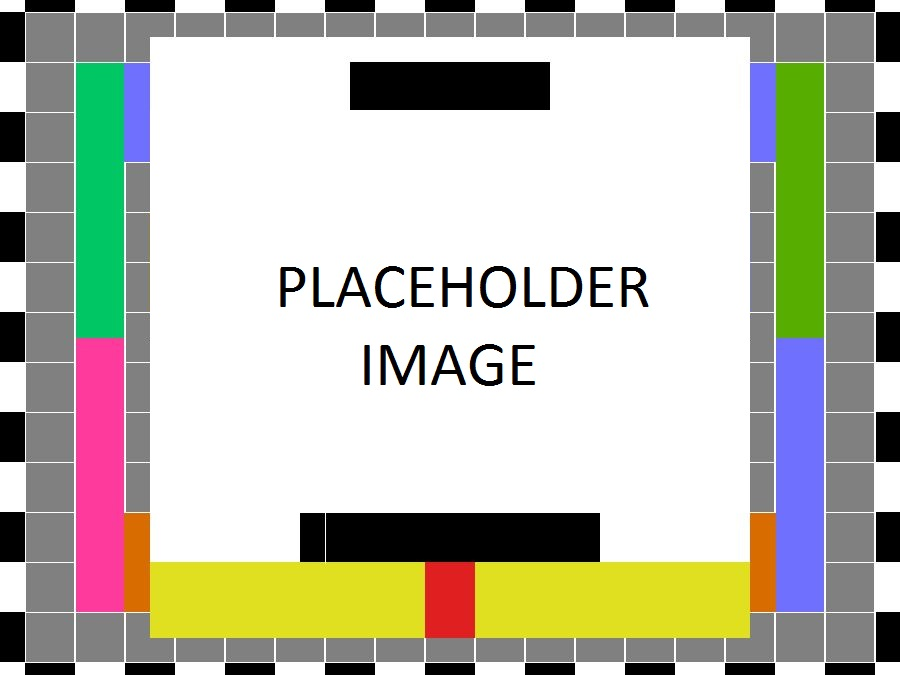
\includegraphics[width=0.60\textwidth]{images/test_image}
\end{figure}
\vspace{0.5 in}
{\centering \huge \color{accentcolor} \sc \textbf{\teamname \\ \productname} \par}
\vspace{0.5 in}
{\centering \large \sc \textbf{\authors} \par}
\newpage


%\vspace{1 in}
%\centerline{January 13th, 2012}
%\newpage

%%% Revision History
\begin{versionhistory}
  	\vhEntry{0.1}{10.01.2015}{GH}{document creation}
  	\vhEntry{0.2}{10.05.2015}{AT|GH}{complete draft}
  	\vhEntry{0.3}{10.12.2015}{AT|GH}{release candidate 1}
  	\vhEntry{1.0}{10.20.2015}{AT|GH|CB}{official release}
  	\vhEntry{1.1}{10.31.2015}{AL}{added design review requests}
\end{versionhistory}
\newpage

%%% Table of contents
\setcounter{tocdepth}{2}
\tableofcontents
\newpage

%%% List of figures and tables (optional)
\listoffigures
\listoftables
\newpage

%%% Document sections
\section{Introduction}
The "Back Burner Brew" is built with the sole purpose of brewing large batch of beer in the home environment. This product provides home brewers with a low-cost electric home brewing system that allow them to have precise control over the brewing process. The brewing process can be automated with the help of micro-controllers like the Raspberry Pi, ESP32 which is then hosted to a local website or an app interface.

ESP32 is a micro-controller that can receive data such as current temperature of the water or mash from the heat sensors located inside the kettles which can be converted to either analog or digital input. The heating coil can be controled using the input from the user as per their desired either to increase or to decrease the temperature. The electric pump can also be controlled by the user through micro-controllers to regulate the flow of the water in the kettles. The user will be able to communicate with the brewing system through a web interface.

The user should expect to input desired commands, controls, and specific
settings such as temperature and length of time through web interface.
The user can expect that whichever temperature they set for their desired
application, that the temperature will remain constant.

The intended audiences for this product would be home brewers or person interested in brewing beer only. Provided that the user manual would be present in the product, any person who wants to brew beer in his local environment can easily use this product. This product is made focusing on how effortless can the brewing process gets simply with the use of micro-controller.
\newpage
\section{System Overview}
This section should describe the overall structure of your software system. Think of it as the strategy for how you will build the system. An architectural "layer" is the top-level logical view, or an abstraction, of your design. Layers should be composed of related elements of similar capabilities, and should be highly independent of other layers, but should have very clearly defined interfaces and interactions with other layers. Each layer should be identified individually and should be unique as to its function and purpose within the system. This section should also contain the high-level block diagram of the layers, as shown in the example below, as well as detailed descriptions of the functions of each layer.

\begin{figure}[H]
	\centering
	\graphicspath{.\images}
	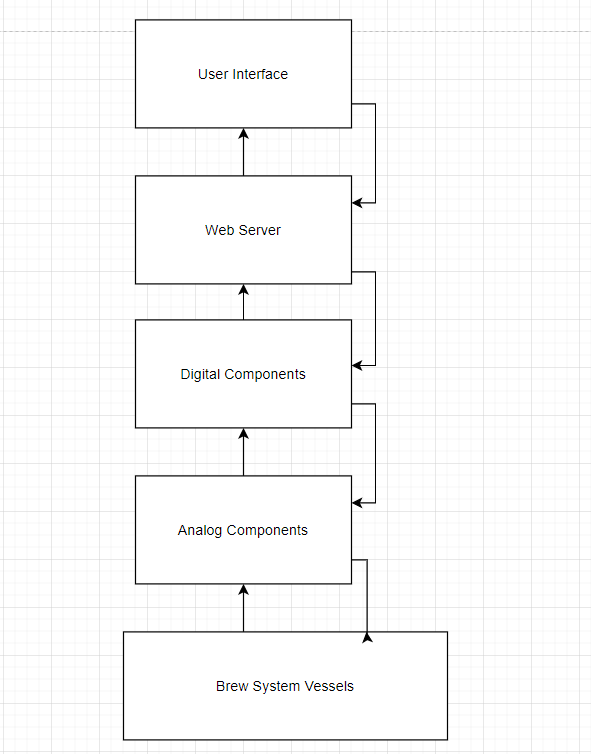
\includegraphics[scale=0.5]{images/simple_ads.PNG}
	\caption{Simple ADS}
\end{figure}
\subsection{Layer X Description}
Each layer should be described separately in detail. Descriptions should include the features, functions, critical interfaces and interactions of the layer. The description should clearly define the services that the layer provides. Also include any conventions that your team will use in describing the structure: naming conventions for layers, subsystems, modules, and data flows; interface specifications; how layers and subsystems are defined; etc. 

\subsection{Layer Y Description}
Each layer should be described separately in detail. Descriptions should include the features, functions, critical interfaces and interactions of the layer. The description should clearly define the services that the layer provides. Also include any conventions that your team will use in describing the structure: naming conventions for layers, subsystems, modules, and data flows; interface specifications; how layers and subsystems are defined; etc. 

\subsection{Layer Z Description}
Each layer should be described separately in detail. Descriptions should include the features, functions, critical interfaces and interactions of the layer. The description should clearly define the services that the layer provides. Also include any conventions that your team will use in describing the structure: naming conventions for layers, subsystems, modules, and data flows; interface specifications; how layers and subsystems are defined; etc. 
\newpage
\section{Subsystem Definitions \& Data Flow}
This section breaks down your layer abstraction to another level of detail. Here you grapically represent the logical subsytems that compose each layer and show the interactions/interfaces between those subsystems. A subsystem can be thought of as a programming unit that implements one of the major functions of the layer. It, therefore, has data elements that serve as source/sinks for other subsystems. The logical data elements that flow between subsystems need to be explicitly defined at this point, beginning with a data flow-like diagram based on the block diagram.

\begin{figure}[H]
	\centering
	\graphicspath{.\images}
	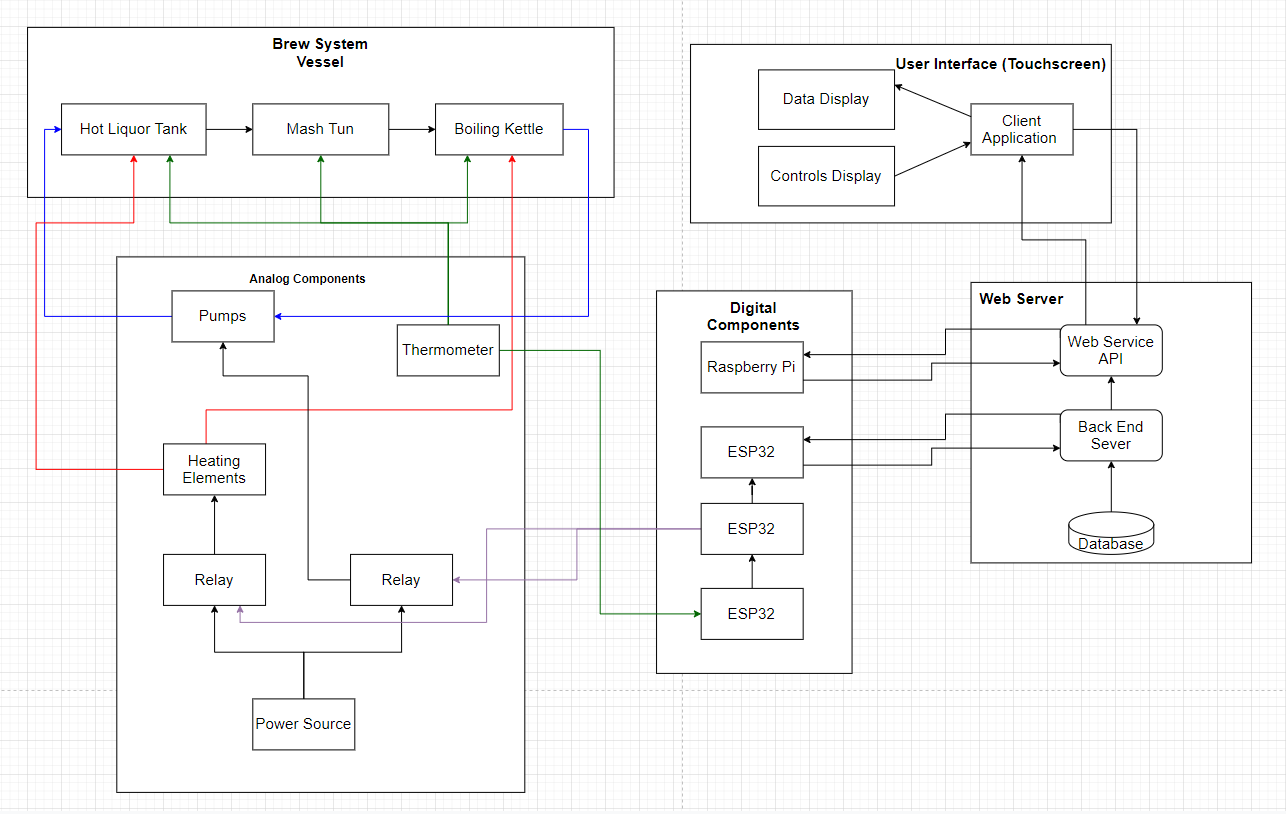
\includegraphics[scale=0.5]{images/ADS_system.PNG}
	\caption{Subsystem ADS}
\end{figure}
\newpage
\section{Brew System Vessel Layer Subsystems}
In this section, the layer is described in some detail in terms of its specific subsystems. Describe each of the layers and its subsystems in a separate chapter/major subsection of this document. The content of each subsystem description should be similar. Include in this section any special considerations and/or trade-offs considered for the approach you have chosen.

The Brewing Vessel layer consists of three major components which plays a vital role in each part for maintaining a good brew. This is the initial phase and the most important layer which should be observed properly. Any mistake made on this layer can drastically affects the taste of beverages. Brew System Vessel layer is directly connected to the some of subsystems from the Analog Components layer which help to regulate the Brewing process. "Brew in A Bag", an alternative for this system was considered which would only contains two subsystems; however, the system chosen in this design provided users with better control and evaluation on overall brewing process. The three subsystems of this layer are explained below:

\begin{figure}[h!]
	\centering
	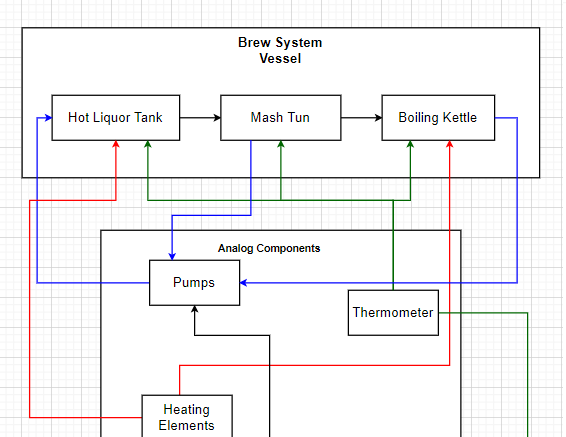
\includegraphics[width=0.60\textwidth]{images/Brew_System_Vessels}
	\caption{Brew System Vessel Layer Representation}
\end{figure}

\subsection{Hot Liquor Tank Subsystem (HLT)}
This section should be a general description of a particular subsystem for the given layer. For most subsystems, an extract of the architectural block diagram with data flows is useful. This should consist of the subsystem being described and those subsystems with which it communicates.

The main purpose of Hot Liquor Tank subsystem is to monitor and heat the water to the desired temperature. This subsystem is directly connected to three subsystems from Analog Components layer which are pumps, thermometer, and heating elements.

\subsubsection{Assumptions}
Any assumptions made in the definition of the subsystem should be listed and described. Pay particular attention to assumptions concerning interfaces and interactions with other layers.

In the initial phase, the vessel should be filled with water by the brewer. The subsystem is controlled by the micro-controller based on the current temperature of the water measured from thermometer and sent through micro-controller to the user.

\subsubsection{Responsibilities}
Each of the responsibilities/features/functions/services of the subsystem as identified in the architectural summary must be expanded to more detailed responsibilities. These responsibilities form the basis for the identification of the finer-grained responsibilities of the layer's internal subsystems. Clearly describe what each subsystem does.

The Hot Liquor Tank subsystem is responsible for providing informations such as current temperature of the water to the brewer, current status of pump and heating elements. Then the subsystem should heat the water to the desired temperature as per the brewer wants. When the water is reached to desired temperature, then it is responsible to pass the water to the Mash Tun subsystem.

\subsubsection{Subsystem Interfaces}
Each of the inputs and outputs for the subsystem are defined here. Create a table with an entry for each labeled interface that connects to this subsystem. For each entry, describe any incoming and outgoing data elements will pass through this interface.

\begin {table}[H]
\caption {Hot Liquor Tank Subsystem interfaces} 
\begin{center}
    \begin{tabular}{| p{0.75cm} | p{6cm} | p{4cm} | p{4cm} |}
    \hline
    ID & Description & Inputs & Outputs \\ \hline
    \#01 & Thermometer Subsystem & \pbox{4cm}{User input to display temperature} & \pbox{4cm}{Current Temperature of the water}  \\ \hline
    \#02 & Pump Subsystem & \pbox{4cm}{User input collected from the micro controller} & \pbox{4cm}{Open/Close the pump based on the input}  \\ \hline
    \#03 & Heating Element Subsystem & \pbox{4cm}{User input in temperature collected from the micro controller} & \pbox{4cm}{Turn on/off heating elements in order to reach user desired temperature }  \\ \hline
    \end{tabular}
\end{center}
\end{table}

\subsection{Mash Tun Subsystem}
The main purpose of Mash Tun subsystem is to mix the hot water with grains to produce wort. This subsystem is directly connected to Thermometer and Pump subsystems from Analog Components layer which is used to provide temperature of the mash.

\subsubsection{Assumptions}
When the Mash Tun is filled with hot water from the HLT, then the Mash Tun is manually loaded with the crushed grains. The user is supposed to set the temperature and time through web or app interface he want the mash to be in this subsystem. If the temperature inside the Mash Tun reached to the different temperature than the user set, the water is sent back to HLT and heated. The mash is rinse several time to rinse the sugar from the mash which is then passed to Boiling Kettle subsystem.


\subsubsection{Responsibilities}
The Mash Tun is responsible to remove sugars, mostly maltose, sucrose and maltotriose from the crushed grains to produce the final product called wort, also known as un-fermented beer. The Mash Tun should provide temperature of the current mash to the brewer. The Mash Tun is responsible to pump out the water to HLT Subsystem when it doesn't maintain required temperature. And when the water is heated enough, then it is again passed to Mash Tun subsystem. By this way, the mash is rinse to get the sugars out. The wort obtained is then passed to Boiling Kettle subsystem in this layer. 

\subsubsection{Subsystem Interfaces}
\begin {table}[H]
\caption {Mash Tun Subsystem interfaces} 
\begin{center}
	\begin{tabular}{| p{0.75cm} | p{6cm} | p{4cm} | p{4cm} |}
		\hline
		ID & Description & Inputs & Outputs \\ \hline
		\#01 & Thermometer Subsystem & \pbox{4cm}{User input to display and set temperature} & \pbox{4cm}{Current Temperature of the mash}  \\ \hline
		\#02 & Pump Subsystem & \pbox{4cm}{User input collected from the micro controller} & \pbox{4cm}{Open/Close the pump based on the temperature of the mash}  \\ \hline
	\end{tabular}
\end{center}
\end{table}

\subsection{Boiling Kettle Subsystem}
The main purpose of Boiling Kettle subsystem is to boil wort for the required amount of time. This subsystem is directly connected to Thermometer, Pump, and Heating elements subsystems from Analog Components layer which is used to maintain the amount of heat provided to the wort.

\subsubsection{Assumptions}
The Boiling Kettle subsystem is almost an automated process. The brewer have to add some hops after each beer cycle in the wort as needed because it add bitterness to the beer. The brewer must be careful with adding appropriate amount of hops as too much can ruin the taste and very little won't bring any taste to beer. 

\subsubsection{Responsibilities}
The Boiling Kettle is only responsible for heating the wort with appropriate heat for the appropriate amount of time. The wort should be heated properly to maintain the good flavor of beer. Once the boil is done, the Boiling Kettle subsystem is responsible for sending beer to the chiller for fermentation.

\subsubsection{Subsystem Interfaces}
\begin {table}[H]
\caption {Boiling Kettle Subsystem interfaces} 
\begin{center}
	\begin{tabular}{| p{0.75cm} | p{6cm} | p{4cm} | p{4cm} |}
		\hline
		ID & Description & Inputs & Outputs \\ \hline
		\#01 & Thermometer Subsystem & \pbox{4cm}{User input to display temperature} & \pbox{4cm}{Current Temperature of the wort}  \\ \hline
		\#02 & Pump Subsystem & \pbox{4cm}{User input collected from the micro controller} & \pbox{4cm}{Open/Close the pump based on the input}  \\ \hline
		\#03 & Heating Element Subsystem & \pbox{4cm}{User input in temperature collected from the micro controller} & \pbox{4cm}{Turn on/off heating elements in order to reach user desired temperature }  \\ \hline
	\end{tabular}
\end{center}
\end{table}


\newpage
\section{Y Layer Subsystems}
In this section, the layer is described in some detail in terms of its specific subsystems. Describe each of the layers and its subsystems in a separate chapter/major subsection of this document. The content of each subsystem description should be similar. Include in this section any special considerations and/or trade-offs considered for the approach you have chosen.

\subsection{Subsystem 1}
This section should be a general description of a particular subsystem for the given layer. For most subsystems, an extract of the architectural block diagram with data flows is useful. This should consist of the subsystem being described and those subsystems with which it communicates.

\begin{figure}[h!]
	\centering
 	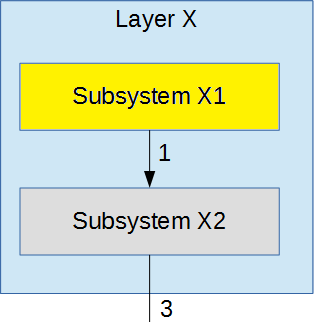
\includegraphics[width=0.60\textwidth]{images/subsystem}
 \caption{Example subsystem description diagram}
\end{figure}

\subsubsection{Assumptions}
Any assumptions made in the definition of the subsystem should be listed and described. Pay particular attention to assumptions concerning interfaces and interactions with other layers.

\subsubsection{Responsibilities}
Each of the responsibilities/features/functions/services of the subsystem as identified in the architectural summary must be expanded to more detailed responsibilities. These responsibilities form the basis for the identification of the finer-grained responsibilities of the layer's internal subsystems. Clearly describe what each subsystem does.

\subsubsection{Subsystem Interfaces}
Each of the inputs and outputs for the subsystem are defined here. Create a table with an entry for each labelled interface that connects to this subsystem. For each entry, describe any incoming and outgoing data elements will pass through this interface.

\begin {table}[H]
\caption {Subsystem interfaces} 
\begin{center}
    \begin{tabular}{ | p{1cm} | p{6cm} | p{3cm} | p{3cm} |}
    \hline
    ID & Description & Inputs & Outputs \\ \hline
    \#xx & Description of the interface/bus & \pbox{3cm}{input 1 \\ input 2} & \pbox{3cm}{output 1}  \\ \hline
    \#xx & Description of the interface/bus & \pbox{3cm}{N/A} & \pbox{3cm}{output 1}  \\ \hline
    \end{tabular}
\end{center}
\end{table}

\subsection{Subsystem 2}
Repeat for each subsystem

\subsection{Subsystem 3}
Repeat for each subsystem


\newpage
\section{Z Layer Subsystems}
In this section, the layer is described in some detail in terms of its specific subsystems. Describe each of the layers and its subsystems in a separate chapter/major subsection of this document. The content of each subsystem description should be similar. Include in this section any special considerations and/or trade-offs considered for the approach you have chosen.

\subsection{Subsystem 1}
This section should be a general description of a particular subsystem for the given layer. For most subsystems, an extract of the architectural block diagram with data flows is useful. This should consist of the subsystem being described and those subsystems with which it communicates.

\begin{figure}[h!]
	\centering
 	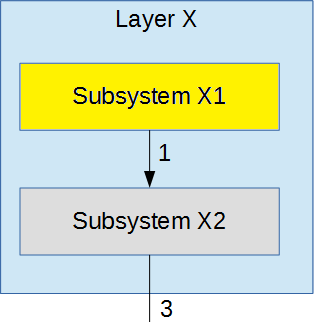
\includegraphics[width=0.60\textwidth]{images/subsystem}
 \caption{Example subsystem description diagram}
\end{figure}

\subsubsection{Assumptions}
Any assumptions made in the definition of the subsystem should be listed and described. Pay particular attention to assumptions concerning interfaces and interactions with other layers.

\subsubsection{Responsibilities}
Each of the responsibilities/features/functions/services of the subsystem as identified in the architectural summary must be expanded to more detailed responsibilities. These responsibilities form the basis for the identification of the finer-grained responsibilities of the layer's internal subsystems. Clearly describe what each subsystem does.

\subsubsection{Subsystem Interfaces}
Each of the inputs and outputs for the subsystem are defined here. Create a table with an entry for each labelled interface that connects to this subsystem. For each entry, describe any incoming and outgoing data elements will pass through this interface.

\begin {table}[H]
\caption {Subsystem interfaces} 
\begin{center}
    \begin{tabular}{ | p{1cm} | p{6cm} | p{3cm} | p{3cm} |}
    \hline
    ID & Description & Inputs & Outputs \\ \hline
    \#xx & Description of the interface/bus & \pbox{3cm}{input 1 \\ input 2} & \pbox{3cm}{output 1}  \\ \hline
    \#xx & Description of the interface/bus & \pbox{3cm}{N/A} & \pbox{3cm}{output 1}  \\ \hline
    \end{tabular}
\end{center}
\end{table}

\subsection{Subsystem 2}
Repeat for each subsystem

\subsection{Subsystem 3}
Repeat for each subsystem


\newpage

%%% References
\bibliographystyle{plain}
\bibliographystyle{reference/IEEEtran_custom}
\bibliography{reference/refs}{}

\end{document}